\documentclass{article}
\usepackage[margin=0.2in,paperwidth=9in,paperheight=4.8in]{geometry}
\pagestyle{empty}
\usepackage{amsmath,amssymb}
\usepackage{tikz}
\usetikzlibrary{shapes.geometric, arrows.meta, positioning, calc}

\begin{document}
\noindent
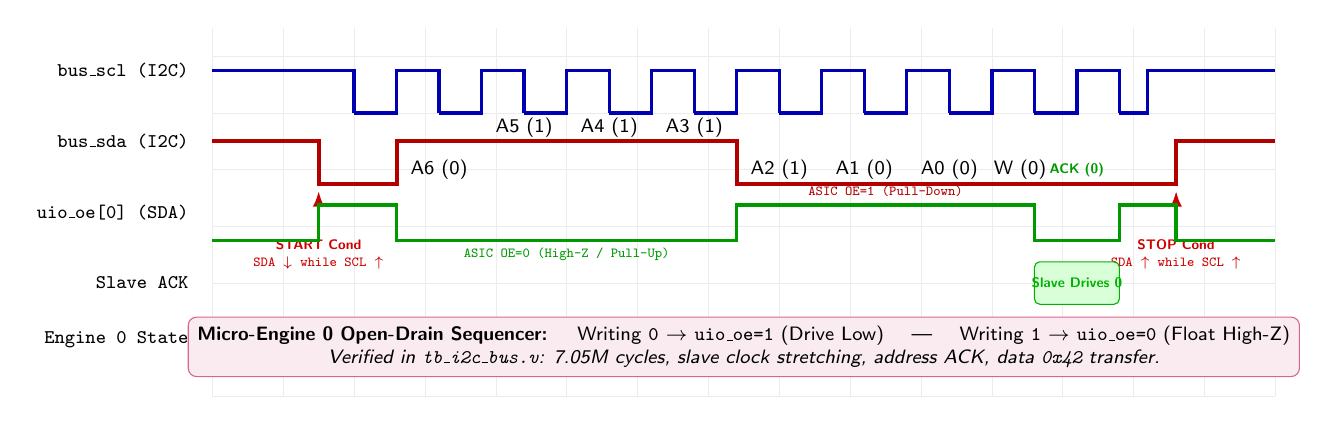
\begin{tikzpicture}[
    scale=0.9,
    clock/.style={line width=1.2pt, blue!70!black},
    sda/.style={line width=1.4pt, red!70!black},
    oe/.style={line width=1.2pt, green!60!black},
    txt/.style={font=\scriptsize\sffamily},
    lbl/.style={font=\scriptsize\ttfamily, anchor=east}
]

% Background grid
\draw[help lines, color=gray!15, ystep=0.8, xstep=1] (0, 0) grid (15, 5.2);

% Labels
\node[lbl] at (-0.2, 4.6) {bus\_scl (I2C)};
\node[lbl] at (-0.2, 3.6) {bus\_sda (I2C)};
\node[lbl] at (-0.2, 2.6) {uio\_oe[0] (SDA)};
\node[lbl] at (-0.2, 1.6) {Slave ACK};
\node[lbl] at (-0.2, 0.8) {Engine 0 State};

% I2C SCL: Idle High -> START -> 9 SCL clocks (7 Addr + R/W + ACK) -> STOP
\draw[clock] (0, 4.6) -- (2.0, 4.6) -- (2.0, 4.0);
\foreach \i in {0,...,8} {
    \draw[clock] (2.0 + \i*1.2, 4.0) -- (2.0 + \i*1.2 + 0.6, 4.0) -- (2.0 + \i*1.2 + 0.6, 4.6) -- (2.0 + \i*1.2 + 1.2, 4.6) -- (2.0 + \i*1.2 + 1.2, 4.0);
}
\draw[clock] (12.8, 4.0) -- (13.2, 4.0) -- (13.2, 4.6) -- (15, 4.6);

% I2C SDA: START condition (falling while SCL high at x=1.5)
% Address: 0x3C = 0111100 + R/W=0 (Write) -> 9th bit = Slave pulls low (ACK)
% Bits: 0, 1, 1, 1, 1, 0, 0, 0 (W), ACK=0
\draw[sda] (0, 3.6) -- (1.5, 3.6) -- (1.5, 3.0) % START condition
          -- (2.6, 3.0) -- (2.6, 3.6) -- (7.4, 3.6) -- (7.4, 3.0) % A6=0, A5..A2=1, A1..A0=0
          -- (11.0, 3.0) % R/W = 0
          -- (12.2, 3.0) % Slave ACK = 0
          -- (12.2, 3.0) -- (13.6, 3.0) -- (13.6, 3.6) -- (15, 3.6); % STOP condition

% Annotations for START and STOP
\draw[-{Latex[length=2mm]}, red!80!black, line width=1pt] (1.5, 2.3) -- (1.5, 2.9);
\node[txt, font=\tiny\bfseries\sffamily, red!80!black, align=center] at (1.5, 2.0) {\textbf{START Cond}\\\texttt{SDA $\downarrow$ while SCL $\uparrow$}};

\draw[-{Latex[length=2mm]}, red!80!black, line width=1pt] (13.6, 2.3) -- (13.6, 2.9);
\node[txt, font=\tiny\bfseries\sffamily, red!80!black, align=center] at (13.6, 2.0) {\textbf{STOP Cond}\\\texttt{SDA $\uparrow$ while SCL $\uparrow$}};

% Bit labels
\node[txt] at (3.2, 3.2) {A6 (0)};
\node[txt] at (4.4, 3.8) {A5 (1)};
\node[txt] at (5.6, 3.8) {A4 (1)};
\node[txt] at (6.8, 3.8) {A3 (1)};
\node[txt] at (8.0, 3.2) {A2 (1)};
\node[txt] at (9.2, 3.2) {A1 (0)};
\node[txt] at (10.4, 3.2) {A0 (0)};
\node[txt] at (11.4, 3.2) {W (0)};
\node[txt, font=\tiny\bfseries\sffamily, green!60!black] at (12.2, 3.2) {ACK (0)};

% uio_oe[0] (Active low pulldown: 1 pulls bus low, 0 releases bus high-Z)
\draw[oe] (0, 2.2) -- (1.5, 2.2) -- (1.5, 2.7) -- (2.6, 2.7) -- (2.6, 2.2)
         -- (7.4, 2.2) -- (7.4, 2.7) -- (11.6, 2.7) -- (11.6, 2.2) % releases at 11.6 for slave ACK
         -- (12.8, 2.2) -- (12.8, 2.7) -- (13.6, 2.7) -- (13.6, 2.2) -- (15, 2.2);
\node[txt, font=\tiny\ttfamily, green!60!black] at (5.0, 2.0) {ASIC OE=0 (High-Z / Pull-Up)};
\node[txt, font=\tiny\ttfamily, red!70!black] at (9.5, 2.9) {ASIC OE=1 (Pull-Down)};

% Slave ACK active indicator
\draw[fill=green!15, draw=green!70!black, rounded corners=2pt] (11.6, 1.3) rectangle (12.8, 1.9);
\node[txt, font=\tiny\bfseries\sffamily, green!70!black] at (12.2, 1.6) {Slave Drives 0};

% Engine State
\node[draw=purple!60, fill=purple!8, rounded corners=3pt, font=\scriptsize\sffamily, align=center] at (7.5, 0.7) {
    \textbf{Micro-Engine 0 Open-Drain Sequencer:} \quad Writing \texttt{0} $\rightarrow$ \texttt{uio\_oe=1} (Drive Low) \quad | \quad Writing \texttt{1} $\rightarrow$ \texttt{uio\_oe=0} (Float High-Z) \\
    \textit{Verified in \texttt{tb\_i2c\_bus.v}: 7.05M cycles, slave clock stretching, address ACK, data \texttt{0x42} transfer.}
};

\end{tikzpicture}
\end{document}
